\documentclass{article}
\linespread{1.3}
\usepackage[margin=50pt]{geometry}
\usepackage{amsmath, amsthm, amssymb, amsthm, tikz, fancyhdr, float, graphicx, spverbatim, systeme}
\pagestyle{fancy}
\renewcommand{\headrulewidth}{0pt}
\newcommand{\changefont}{\fontsize{15}{15}\selectfont}

\fancypagestyle{firstpageheader}{
  \fancyhead[R]{
    \changefont
    \parbox[t]{4cm}{ % Adjust width as needed
      Michael Huang\\
      EN.625.633.81\\
      Homework 11
    }
  }
}

\begin{document}

\thispagestyle{firstpageheader}
{\Large 

\section*{1.}

\subsection*{(a)}



\subsection*{(b)}



}
{\Large 

\section*{2.}

\subsection*{(a)}



\subsection*{(b)}



}
{\Large 

\section*{3.}

We aim to find the number of bootstraps necessary to accurately calculate a 95\% confidence interval in the difference of two population means. \\ \\ 
The plan is to simulate \(n\) values of \(X_1 \sim N(\mu_1, \sigma_1^2)\) and \(m\) values of \(Y \sim N(\mu_2, \sigma^2)\) and calculate a 95\% confidence interval in \(\mu_1 - \mu_2\). Then, calculate a 95\% confidence interval for \(\mu_1 - \mu_2\) using the bootstrap techniques learned in the module, that is: \\
- Sample bootstramp sample \(X^*\) with replacement \\
- Sample bootstrap sample \(Y^*\) with replacement \\
- Calculate \(\mu_1 - \mu_2\) for each bootstrap sample \\
- Take the 95\% confidence interval in the middle as normal \\
\begin{spverbatim}
> B_values = c(100, 500, 1000, 2500, 5000, 10000)
> # Repeat multiple times to get to steady state
> repetitions = 100
> 
> n = 50
> mu_1 = 3
> sigma_1 = 1
> 
> m = 50
> mu_2 = 4
> sigma_2 = 2
> 
> X = rnorm(n, mean = mu_1, sd = sigma_1)
> Y = rnorm(m, mean = mu_2, sd = sigma_2)
> 
> # For calculated CI, use Welch's t-test which does not assume equal variances
> normal_t_test = t.test(X, Y, conf.level = 0.95)
> calculated_ci = normal_t_test$conf.int
> 
> bootstrap_ci = function(X, Y, B) {
+   bootstrap_differences = rep(0, B)
+   for (j in 1:B) {
+     boot_x = sample(X, n, replace = TRUE)
+     boot_y = sample(Y, m, replace = TRUE)
+     
+     bootstrap_differences[j] = mean(boot_x) - mean(boot_y)
+   }
+   
+   bootstrap_ci = quantile(bootstrap_differences, probs = c(0.025, 0.975))
+   
+ }
> 
> bootstrap_results = data.frame(B = integer(), ci_lower = numeric(), ci_upper = numeric())
> for (B in B_values) {
+   
+   lower_results = rep(0, repetitions)
+   upper_results = rep(0, repetitions)
+   for (r in 1:repetitions) {
+     bootstrap_result = bootstrap_ci(X, Y, B)
+     lower_results[r] = bootstrap_result[1]
+     upper_results[r] = bootstrap_result[2]
+   }
+   
+   bootstrap_results = rbind(bootstrap_results, data.frame(
+     B = B,
+     lower_mean = mean(lower_results),
+     lower_sd = sd(lower_results),
+     upper_mean = mean(upper_results),
+     upper_sd = sd(upper_results)
+   ))
+ }
> 
> sprintf("Calculated CI: [%f, %f]", calculated_ci[1], calculated_ci[2])
[1] "Calculated CI: [-1.716995, -0.326697]"
> 
> print(bootstrap_results)
      B lower_mean    lower_sd upper_mean    upper_sd
1   100  -1.674224 0.081550883 -0.3683828 0.075172619
2   500  -1.697692 0.035720486 -0.3540524 0.041719129
3  1000  -1.692301 0.030432004 -0.3520838 0.028434478
4  2500  -1.698923 0.017086303 -0.3496306 0.018933560
5  5000  -1.699331 0.013708461 -0.3500792 0.012151156
6 10000  -1.700329 0.008748158 -0.3493192 0.008897934
>
> # Lower means, normal and log
> par(mfrow = c(1, 2))
> plot(bootstrap_results$B, bootstrap_results$lower_mean,
+      type = "b", 
+      ylim = range(c(bootstrap_results$lower_mean - bootstrap_results$lower_sd,
+                     bootstrap_results$lower_mean + bootstrap_results$lower_sd)),
+      xlab = "B", 
+      ylab = "Mean of CI lower bound",
+      main = "CI Lower Bound Mean over B")
> arrows(bootstrap_results$B,
+        bootstrap_results$lower_mean - bootstrap_results$lower_sd,
+        bootstrap_results$B,
+        bootstrap_results$lower_mean + bootstrap_results$lower_sd,
+        code=0
+ )
> abline(h = calculated_ci[1], col = "red")
> plot(bootstrap_results$B, bootstrap_results$lower_mean,
+      type = "b", 
+      log = "x",
+      ylim = range(c(bootstrap_results$lower_mean - bootstrap_results$lower_sd,
+                     bootstrap_results$lower_mean + bootstrap_results$lower_sd)),
+      xlab = "B (log scale)", 
+      ylab = "Mean of CI lower bound",
+      main = "CI Lower Bound Mean over B (log scale)")
> arrows(bootstrap_results$B,
+        bootstrap_results$lower_mean - bootstrap_results$lower_sd,
+        bootstrap_results$B,
+        bootstrap_results$lower_mean + bootstrap_results$lower_sd,
+        code=0
+ )
> abline(h = calculated_ci[1], col = "red")
> 
> # Lower SDs, normal and log
> par(mfrow = c(1, 2))
> plot(bootstrap_results$B, bootstrap_results$lower_sd,
+      type = "b", 
+      xlab = "B", 
+      ylab = "SD of CI lower bound",
+      main = "CI Lower Bound SD over B")
> plot(bootstrap_results$B, bootstrap_results$lower_sd,
+      type = "b", 
+      log = "x",
+      xlab = "B (log scale)", 
+      ylab = "SD of CI lower bound",
+      main = "CI Lower Bound SD over B (log scale)")
> 
> # Upper means, normal and log
> par(mfrow = c(1, 2))
> plot(bootstrap_results$B, bootstrap_results$upper_mean,
+      type = "b", 
+      ylim = range(c(bootstrap_results$upper_mean - bootstrap_results$upper_sd,
+                     bootstrap_results$upper_mean + bootstrap_results$upper_sd)),
+      xlab = "B", 
+      ylab = "Mean of CI Upper Bound",
+      main = "CI Upper Bound Mean over B")
> arrows(bootstrap_results$B,
+        bootstrap_results$upper_mean - bootstrap_results$upper_sd,
+        bootstrap_results$B,
+        bootstrap_results$upper_mean + bootstrap_results$upper_sd,
+        code=0
+ )
> abline(h = calculated_ci[2], col = "red")
> plot(bootstrap_results$B, bootstrap_results$upper_mean,
+      type = "b", 
+      log = "x",
+      ylim = range(c(bootstrap_results$upper_mean - bootstrap_results$upper_sd,
+                     bootstrap_results$upper_mean + bootstrap_results$upper_sd)),
+      xlab = "B (log scale)", 
+      ylab = "Mean of CI Upper Bound",
+      main = "CI Upper Bound Mean over B (log scale)")
> arrows(bootstrap_results$B,
+        bootstrap_results$upper_mean - bootstrap_results$upper_sd,
+        bootstrap_results$B,
+        bootstrap_results$upper_mean + bootstrap_results$upper_sd,
+        code=0
+ )
> abline(h = calculated_ci[2], col = "red")
> 
> # Upper SDs, normal and log
> par(mfrow = c(1, 2))
> plot(bootstrap_results$B, bootstrap_results$upper_sd,
+      type = "b",
+      xlab = "B", 
+      ylab = "SD of CI Upper Bound",
+      main = "CI Upper Bound SD over B")
> plot(bootstrap_results$B, bootstrap_results$upper_sd,
+      type = "b", 
+      log = "x",
+      xlab = "B (log scale)", 
+      ylab = "SD of CI Upper Bound",
+      main = "CI Upper Bound SD over B (log scale)")
\end{spverbatim}
\begin{figure}[H]
    \centering
    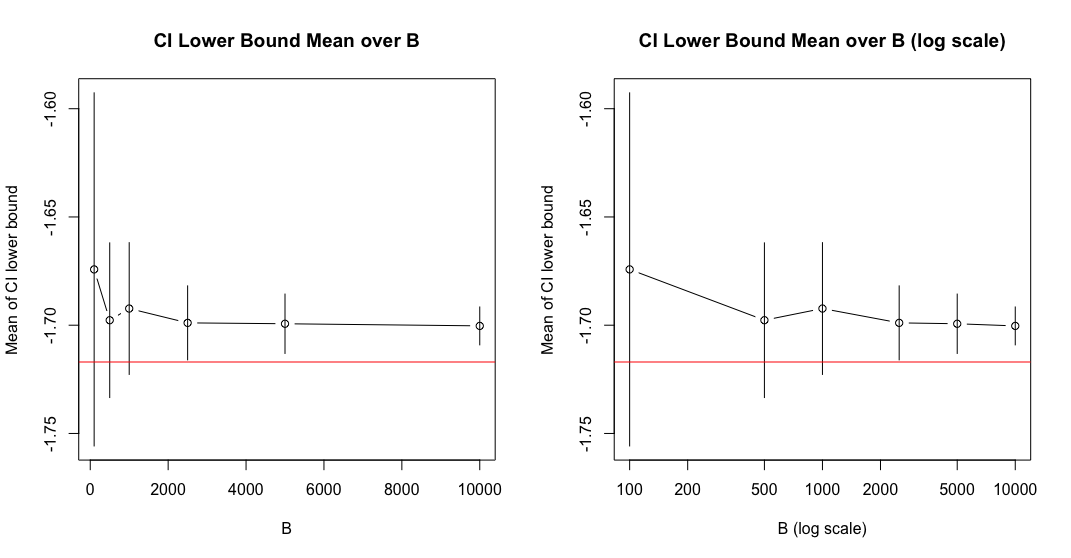
\includegraphics[width=1\textwidth]{problem_3_ci_lower_mean.png}
\end{figure}
\begin{figure}[H]
    \centering
    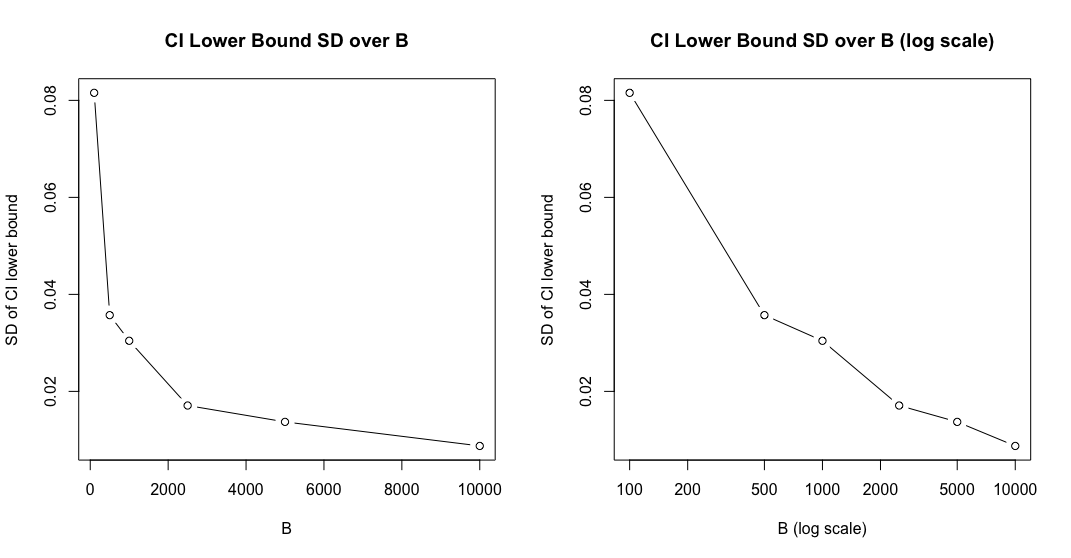
\includegraphics[width=1\textwidth]{problem_3_ci_lower_sd.png}
\end{figure}
\begin{figure}[H]
    \centering
    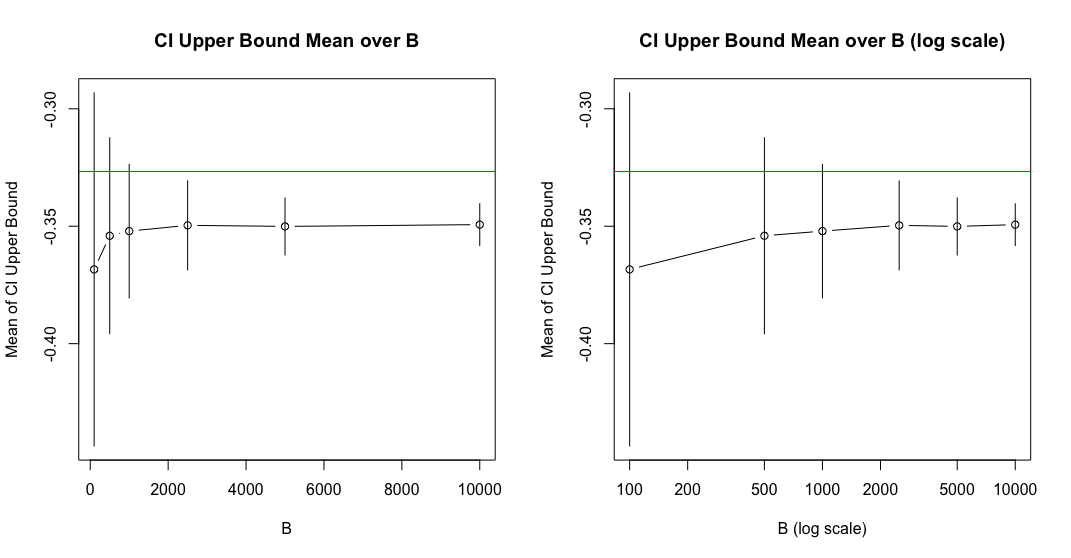
\includegraphics[width=1\textwidth]{problem_3_ci_upper_mean.png}
\end{figure}
\begin{figure}[H]
    \centering
    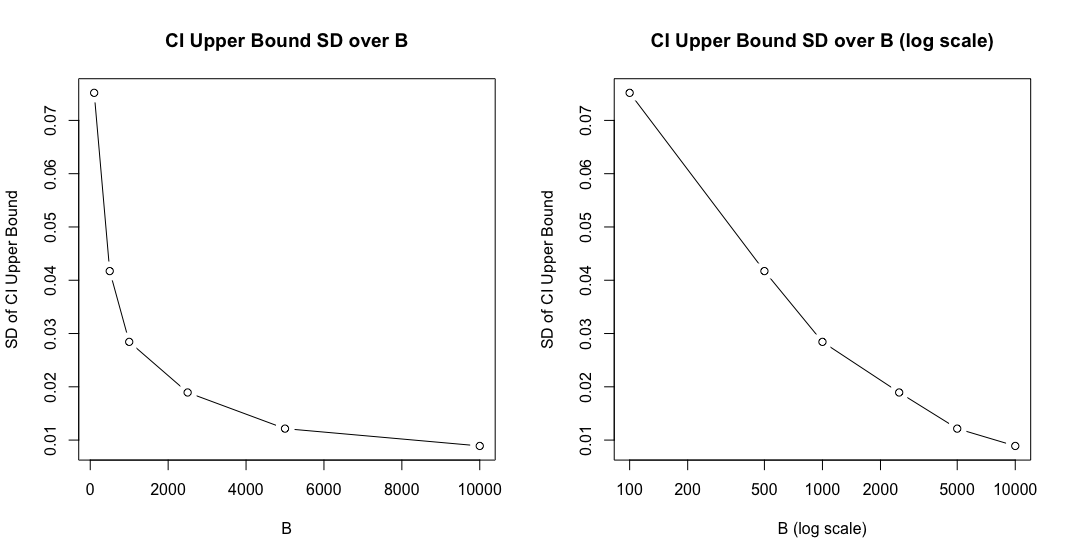
\includegraphics[width=1\textwidth]{problem_3_ci_upper_sd.png}
\end{figure}
Looking at the figures and results, we see that there are generally diminishing returns in terms of getting meaningfully reduced range of mean differences past the \(B = 2500\) point. The SD does continue to improve, however. Clearly, \(B = 100\) is not enough, \(B = 500\) is a decent improvement, and then it begins to become better but in diminishing amounts as we approach \(B = 2500\). This makes sense, given how the bootstrap works relative to a theoretically calculated amount. In my opinion, the threshold seems good around there, however, with the red lines of the calculated bounds, it is notable that the bootstrap will never reach the point of exactly becoming dependably exactly as accurate as the theoretical mean bounds. This makes sense, given the point of using bootstrap and the tradeoff here, so my \(B\) value evaluation criteria was more geared toward hitting a point of relative accuracy is getting as close as we can seemingly get very dependably.


}

\end{document}